\section{Regressore}

\subsection{Dataset originale}

\subsubsection{Dataset completo}

Il nuovo dataset presenta i seguenti valori:
\begin{itemize}
    \item \textbf{n\_users}: [19841, 22155, 23679, 50000, 6040]
    \item \textbf{n\_items}: [42457, 24878, 33653, 38932, 54458, 4414, 10000 3706]
    \item \textbf{n\_inter}: [900212, 218457, 440620, 667850, 1465871, 1048575, 7053774, 1000209]
    \item \textbf{sparsity}: [0.99893136, 0.99955742, 0.9993401, 0.99913541, 0.99878504, 0.98996762,
    0.98589245, 0.95531637]
    \item \textbf{kg\_entities}: [50665, 32907, 42031, 47308, 26315, 0, 175646, 79347]
    \item \textbf{kg\_relations}: [5, 16, 0, 31, 49]
    \item \textbf{kg\_triples}: [46827, 29822, 38491, 43559, 96476, 0, 521125, 385923]
    \item \textbf{kg\_items}: [816701, 11446, 0, 10601, 3655]
    \item \textbf{cpu\_cores}: [12, 4]
    \item \textbf{ram\_size}: [64, 16, 27.40581512]
    \item \textbf{is\_gpu}: [1, 0]
\end{itemize}

\noindent Si può dunque notare un miglioramento per quanto riguarda la varietà dei valori rispetto al passato

\noindent I nuovi dati hanno portato alla seguente distribuzione dei dati (qui di seguito visualizzata):
\begin{figure}[H]
    \centering
    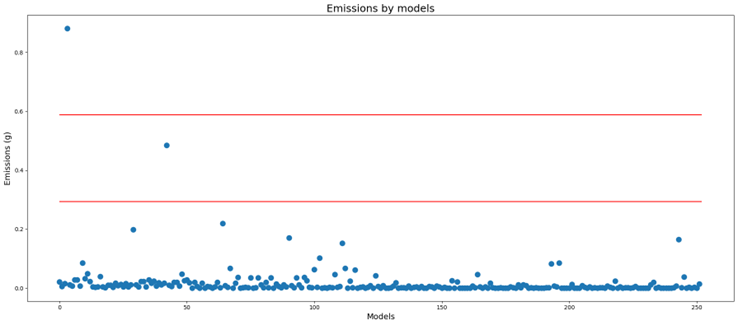
\includegraphics[scale=0.25]{images/nuova-situazione.png}
    \caption{Distribuzione delle emissioni nel dataset completo}
\end{figure}

\noindent Come è possibile notare però, i nuovi esperimenti hanno portato a un'ulteriore sbilanciamento nel dataset, in quanto tutti gli esperimenti con DGCF e altri modelli svettano sui risultati degli altri modelli in emissioni.
Questo si riflette nei risultati ottenuti dai modelli di regressione

\begin{table}[H]
    \centering
    \begin{tabular}{|>{\centering\arraybackslash}m{5cm}|c|c|c|c|}
        \hline
        \textbf{Regressor} & \textbf{MAE} & \textbf{RMSE} & \textbf{MSLE} \\ [10pt]
        \hline
        SVR & 0.1103392 & 0.0268736 & 0.0154947 \\ [10pt]
        \hline
        Decision Tree & 0.0419923 & 0.0139534 & 0.0067713 \\ [10pt]
        \hline
        Random Forest & 0.0410102 & 0.0179366 & 0.0081916 \\ [10pt]
        \hline
        AdaBoost & 0.0486434 & 0.0160941 & 0.0074143 \\ [10pt]
        \hline
    \end{tabular}
    \caption{Risultati ottenuti con il nuovo dataset}
    \label{tab:results} 
\end{table}

\begin{table}[H]
    \centering
    \footnotesize
    \setlength\tabcolsep{0pt}
    \begin{tabularx}{\textwidth}{|X|X|}
        \hline
        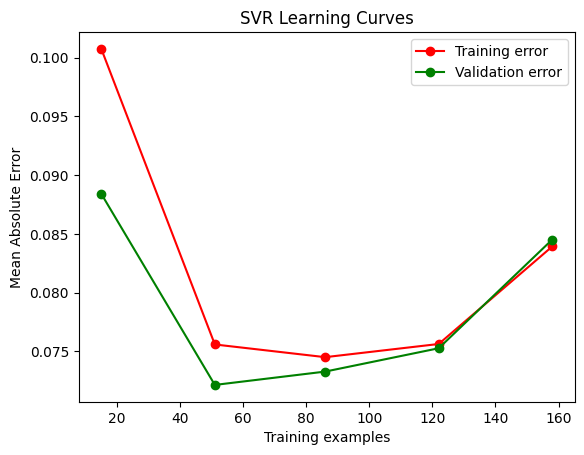
\includegraphics[width=\linewidth, trim=0 0 0 0]{images/SVR_lc2.png} &
        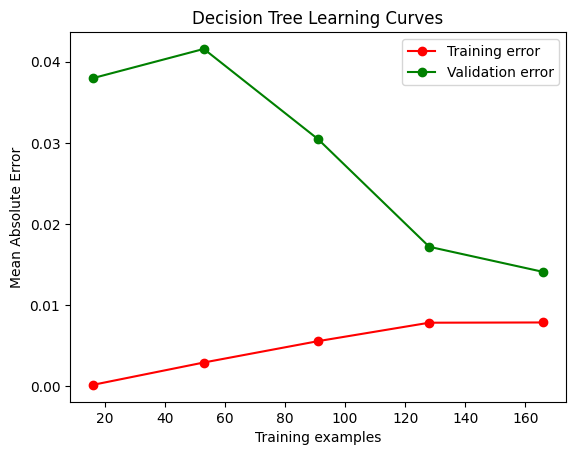
\includegraphics[width=\linewidth, trim=0 0 0 0]{images/DecisionTree_lc2.png} \\
        \hline
        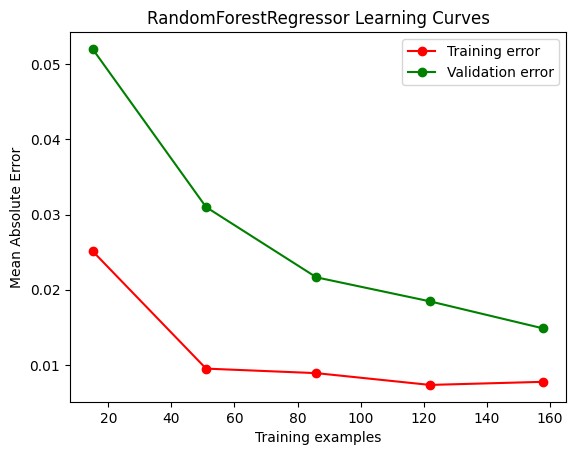
\includegraphics[width=\linewidth, trim=0 0 0 0]{images/RandomForestRegressor_lc2.png} &
        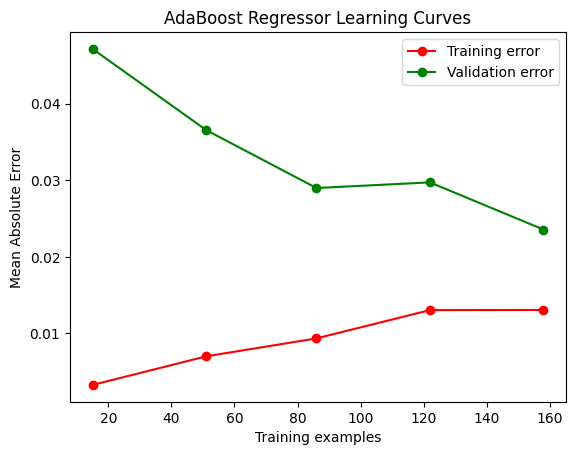
\includegraphics[width=\linewidth, trim=0 0 0 0]{images/AdaBoostRegressor_lc2.png} \\
        \hline
    \end{tabularx}
    \caption{Learning Curves con il nuovo dataset}
    \label{tab:emissions_info}
\end{table}

\noindent E' possibile notare che il forte sbilanciamento nelle emissioni porta i modelli a non apprendere bene. I migliori si riconfermano DecisionTree e RandomForest.

\newpage

\subsubsection{Dataset Azure}

\noindent Una possibile soluzione è stata quella di eliminare tutti i risultati non prodotti sulla macchina Azure. Questo ha portato a un peggioramento dei risultati rispetto al dataset completo

\begin{figure}[H]
    \centering
    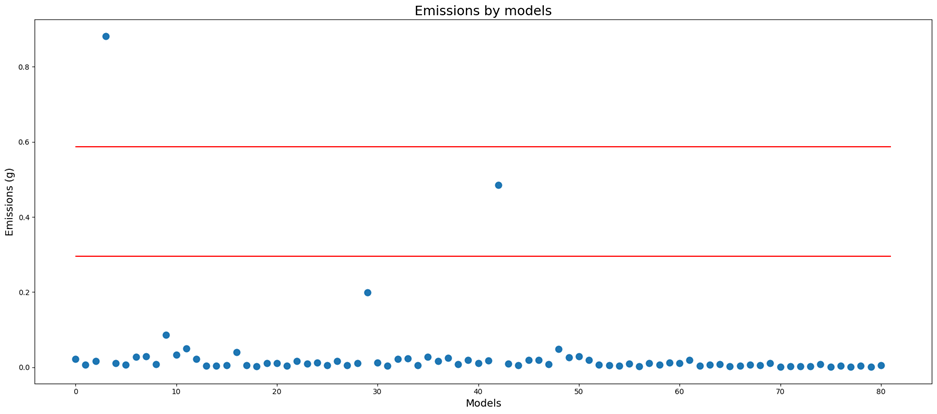
\includegraphics[scale=0.25]{images/nuova-situazione2.png}
    \caption{Distribuzione delle emissioni nel dataset Azure}
\end{figure}


\begin{table}[H]
    \centering
    \begin{tabular}{|>{\centering\arraybackslash}m{5cm}|c|c|c|c|}
        \hline
        \textbf{Regressor} & \textbf{MAE} & \textbf{RMSE} & \textbf{MSLE} \\ [10pt]
        \hline
        SVR & 0.1165169 & 0.0301642 & 0.0175917 \\ [10pt]
        \hline
        Decision Tree & 0.0691471 & 0.0450743 & 0.0199880 \\ [10pt]
        \hline
        Random Forest & 0.0641987 & 0.0306766 & 0.0153200 \\ [10pt]
        \hline
        AdaBoost & 0.0910959 & 0.0542499 & 0.0254505 \\ [10pt]
        \hline
    \end{tabular}
    \caption{Risultati ottenuti con il nuovo dataset Azure}
    \label{tab:results}
\end{table}

\begin{table}[H]
    \centering
    \footnotesize
    \setlength\tabcolsep{0pt}
    \begin{tabularx}{\textwidth}{|X|X|}
        \hline
        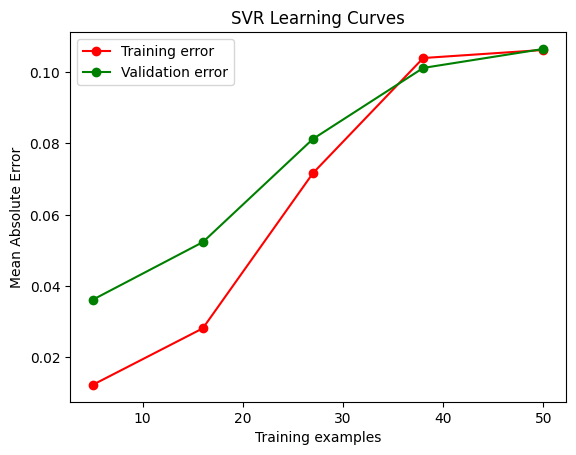
\includegraphics[width=\linewidth, trim=0 0 0 0]{images/SVR_Azure_lc2.png} &
        \includegraphics[width=\linewidth, trim=0 0 0 0]{images/DecisionTree_Azure_lc2.png} \\
        \hline
        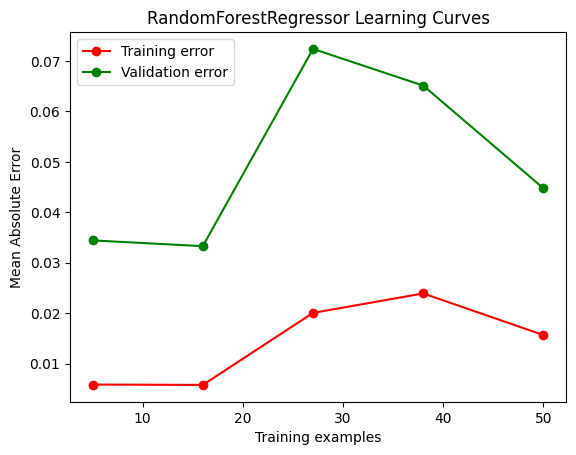
\includegraphics[width=\linewidth, trim=0 0 0 0]{images/RandomForestRegressor_Azure_lc2.png} &
        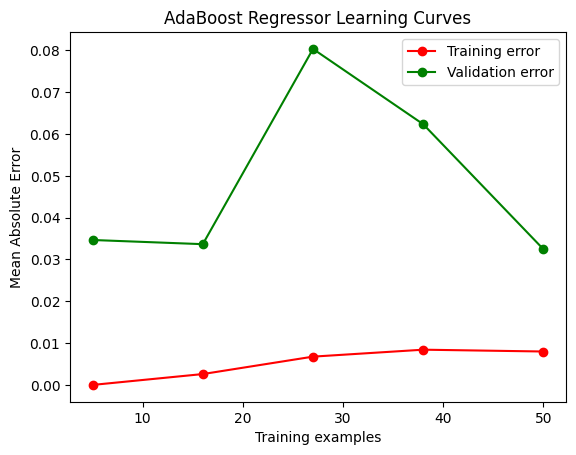
\includegraphics[width=\linewidth, trim=0 0 0 0]{images/AdaBoostRegressor_Azure_lc2.png} \\
        \hline
    \end{tabularx}
    \caption{Learning Curves con il nuovo dataset Azure}
    \label{tab:emissions_info}
\end{table}

\noindent Si riscontrano gli stessi problemi del dataset completo
\newpage

\subsection{Dataset ridotto}

Per provare a migliorare ancor di più le performance dei modelli di regressione, si è deciso di eliminare tutti gli outlier dal dataset(in questo caso le emissioni più alte). In particolare si sono eliminate 11 emissioni dal dataset completo e 8 dal dataset AZURE.

\subsubsection{Dataset completo ridotto}

\begin{figure}[H]
    \centering
    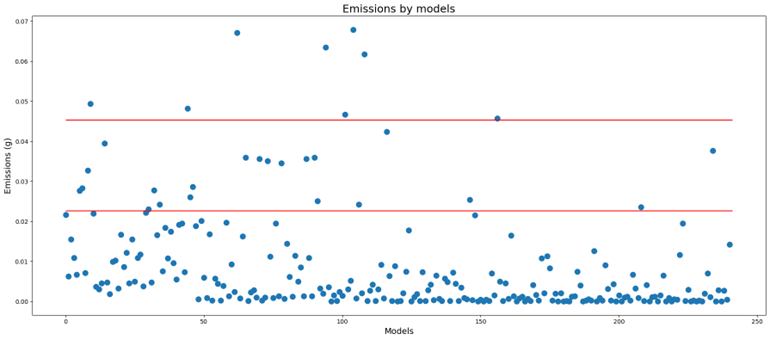
\includegraphics[scale=0.25]{images/nuova-situazione-ridotto.png}
    \caption{Distribuzione delle emissioni nel dataset completo ridotto}
\end{figure}

E' possibile notare un miglior bilanciamento delle emissioni. Per quanto riguarda i modelli, sono stati eseguti addestramenti con diversi split tra training e test set

\noindent\textbf{Split 50/50}


\begin{table}[H]
    \centering
    \begin{tabular}{|>{\centering\arraybackslash}m{5cm}|c|c|c|c|}
        \hline
        \textbf{Regressor} & \textbf{MAE} & \textbf{RMSE} & \textbf{MSLE} \\ [10pt]
        \hline
        SVR & 0.0357360 & 0.0014172 & 0.0013505 \\ [10pt]
        \hline
        Decision Tree & 0.0071074 & 0.0001741 & 0.0001635 \\ [10pt]
        \hline
        Random Forest & 0.0067896 & 0.0001391 & 0.0001312 \\ [10pt]
        \hline
        AdaBoost & 0.0080218 & 0.0001498 & 0.0001417 \\ [10pt]
        \hline
    \end{tabular}
    \caption{Risultati regressore con dataset completo ridotto 50/50}
    \label{tab:results}
\end{table}

\begin{table}[H]
    \centering
    \footnotesize
    \setlength\tabcolsep{0pt}
    \begin{tabularx}{\textwidth}{|X|X|}
        \hline
        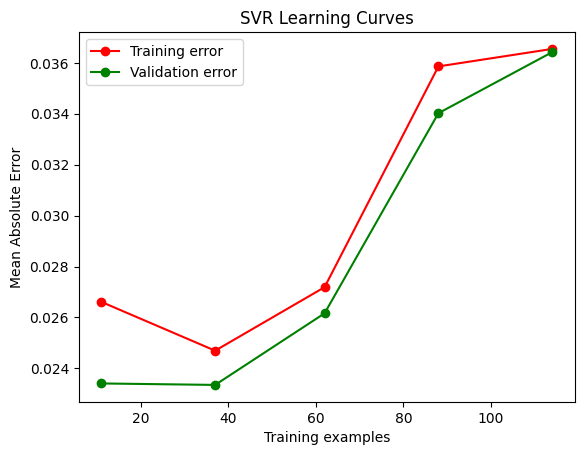
\includegraphics[width=\linewidth, trim=0 0 0 0]{images/SVR_lc50_ridotto.png} &
        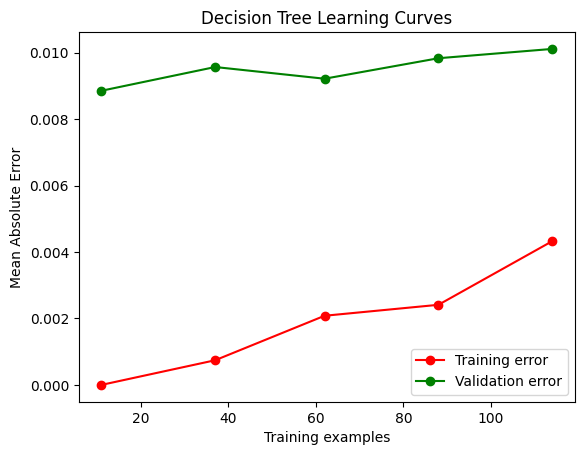
\includegraphics[width=\linewidth, trim=0 0 0 0]{images/DecisionTree_lc50_ridotto.png} \\
        \hline
        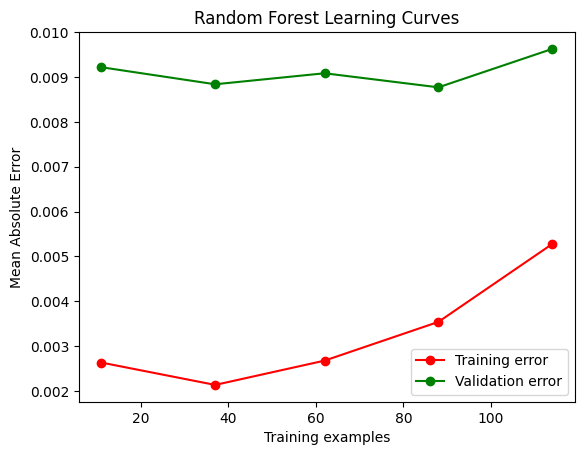
\includegraphics[width=\linewidth, trim=0 0 0 0]{images/RandomForest_lc50_ridotto.png} &
        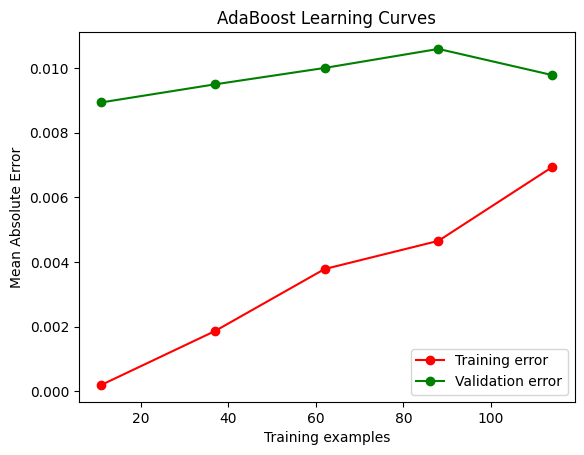
\includegraphics[width=\linewidth, trim=0 0 0 0]{images/AdaBoost_lc50_ridotto.png} \\
        \hline
    \end{tabularx}
    \caption{Learning Curves con dataset completo ridotto 50/50}
    \label{tab:emissions_info}
\end{table}

\noindent RandomForest sembrerebbe essere il migliore


\noindent\textbf{Split 60/40}


\begin{table}[H]
    \centering
    \begin{tabular}{|>{\centering\arraybackslash}m{5cm}|c|c|c|c|}
        \hline
        \textbf{Regressor} & \textbf{MAE} & \textbf{RMSE} & \textbf{MSLE} \\ [10pt]
        \hline
        SVR & 0.0351053 & 0.0013804 & 0.0013161 \\ [10pt]
        \hline
        Decision Tree & 0.0072612 & 0.0001487 & 0.0001409 \\ [10pt]
        \hline
        Random Forest & 0.0064122 & 0.0000973 & 0.0000930 \\ [10pt]
        \hline
        AdaBoost & 0.0088515 & 0.0001644 & 0.0001578 \\ [10pt]
        \hline
    \end{tabular}
    \caption{Risultati regressore con dataset completo ridotto 60/40}
    \label{tab:results}
\end{table}


\begin{table}[H]
    \centering
    \footnotesize
    \setlength\tabcolsep{0pt}
    \begin{tabularx}{\textwidth}{|X|X|}
        \hline
        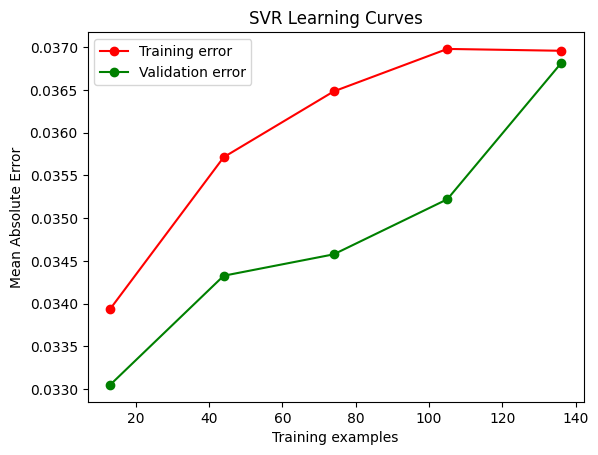
\includegraphics[width=\linewidth, trim=0 0 0 0]{images/SVR_lc60_ridotto.png} &
        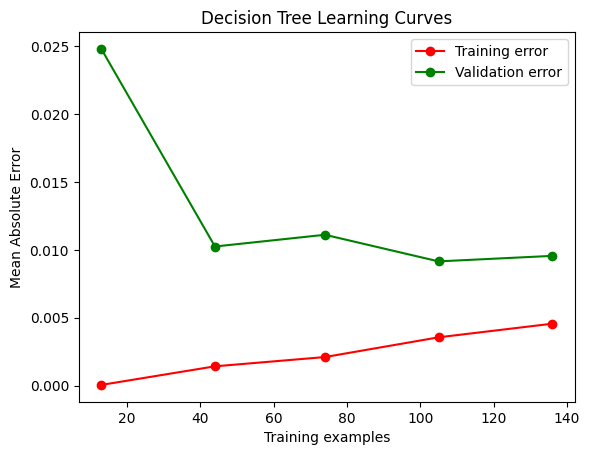
\includegraphics[width=\linewidth, trim=0 0 0 0]{images/DecisionTree_lc60_ridotto.png} \\
        \hline
        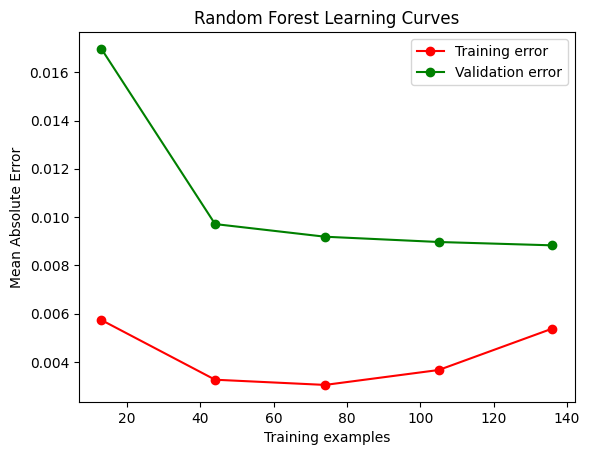
\includegraphics[width=\linewidth, trim=0 0 0 0]{images/RandomForest_lc60_ridotto.png} &
        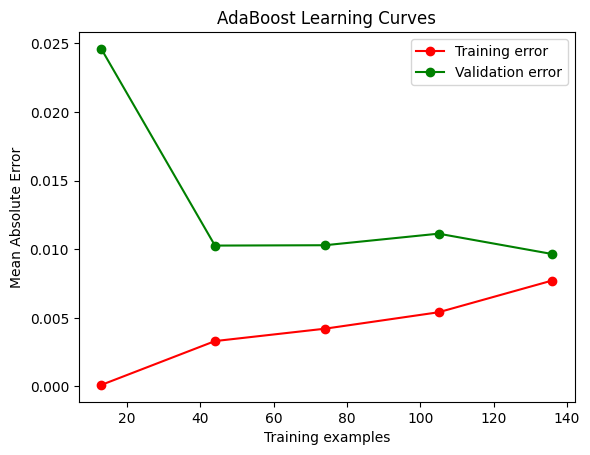
\includegraphics[width=\linewidth, trim=0 0 0 0]{images/AdaBoost_lc60_ridotto.png} \\
        \hline
    \end{tabularx}
    \caption{Learning Curves con dataset completo ridotto 60/40}
    \label{tab:emissions_info}
\end{table}

\noindent RandomForest sembrerebbe essere il migliore

\noindent\textbf{Split 70/30}


\begin{table}[H]
    \centering
    \begin{tabular}{|>{\centering\arraybackslash}m{5cm}|c|c|c|c|}
        \hline
        \textbf{Regressor} & \textbf{MAE} & \textbf{RMSE} & \textbf{MSLE} \\ [10pt]
        \hline
        SVR & 0.0351675 & 0.0013755 & 0.0013111 \\ [10pt]
        \hline
        Decision Tree & 0.0066729 & 0.0001254 & 0.0001196 \\ [10pt]
        \hline
        Random Forest & 0.0067262 & 0.0001148 & 0.0001100 \\ [10pt]
        \hline
        AdaBoost & 0.0080581 & 0.0001397 & 0.0001339 \\ [10pt]
        \hline
    \end{tabular}
    \caption{Risultati regressore con dataset completo ridotto 70/30}
    \label{tab:results}
\end{table}

\begin{table}[H]
    \centering
    \footnotesize
    \setlength\tabcolsep{0pt}
    \begin{tabularx}{\textwidth}{|X|X|}
        \hline
        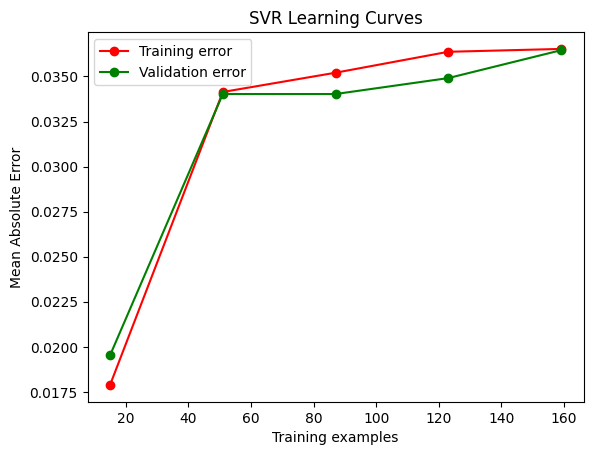
\includegraphics[width=\linewidth, trim=0 0 0 0]{images/SVR_lc70_ridotto.png} &
        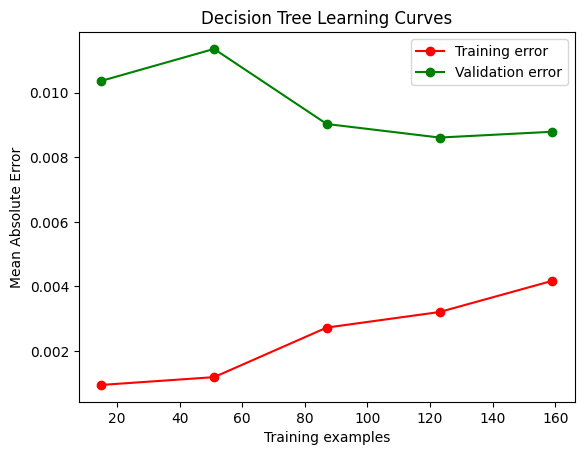
\includegraphics[width=\linewidth, trim=0 0 0 0]{images/DecisionTree_lc70_ridotto.png} \\
        \hline
        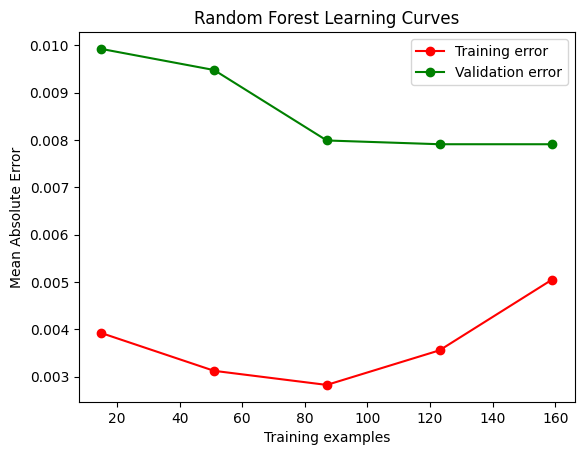
\includegraphics[width=\linewidth, trim=0 0 0 0]{images/RandomForest_lc70_ridotto.png} &
        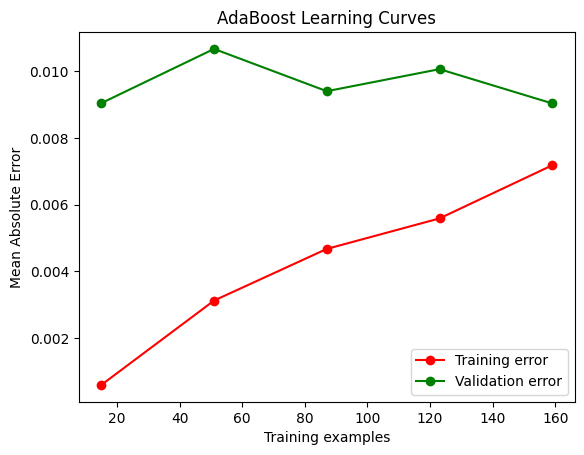
\includegraphics[width=\linewidth, trim=0 0 0 0]{images/AdaBoost_lc70_ridotto.png} \\
        \hline
    \end{tabularx}
    \caption{Learning Curves con dataset completo ridotto 70/30}
    \label{tab:emissions_info}
\end{table}

\noindent RandomForest sembrerebbe essere il migliore


\noindent\textbf{Split 80/20}


\begin{table}[H]
    \centering
    \begin{tabular}{|>{\centering\arraybackslash}m{5cm}|c|c|c|c|}
        \hline
        \textbf{Regressor} & \textbf{MAE} & \textbf{RMSE} & \textbf{MSLE} \\ [10pt]
        \hline
        SVR & 0.0344696 & 0.0013440 & 0.0012808 \\ [10pt]
        \hline
        Decision Tree & 0.0074149 & 0.0001473 & 0.0001397 \\ [10pt]
        \hline
        Random Forest & 0.0069751 & 0.0001199 & 0.0001140 \\ [10pt]
        \hline
        AdaBoost & 0.0094008 & 0.0001633 & 0.0001562 \\ [10pt]
        \hline
    \end{tabular}
    \caption{Risultati regressore con dataset completo ridotto 80/20}
    \label{tab:results}
\end{table}

\begin{table}[H]
    \centering
    \footnotesize
    \setlength\tabcolsep{0pt}
    \begin{tabularx}{\textwidth}{|X|X|}
        \hline
        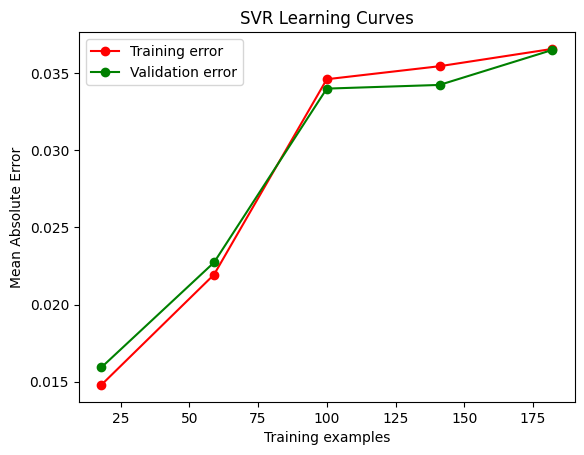
\includegraphics[width=\linewidth, trim=0 0 0 0]{images/SVR_lc80_ridotto.png} &
        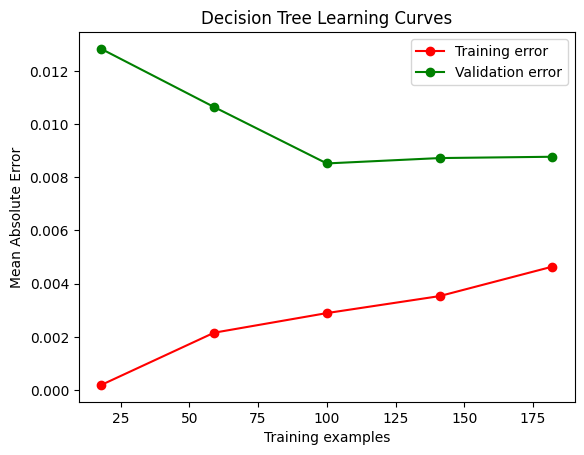
\includegraphics[width=\linewidth, trim=0 0 0 0]{images/DecisionTree_lc80_ridotto.png} \\
        \hline
        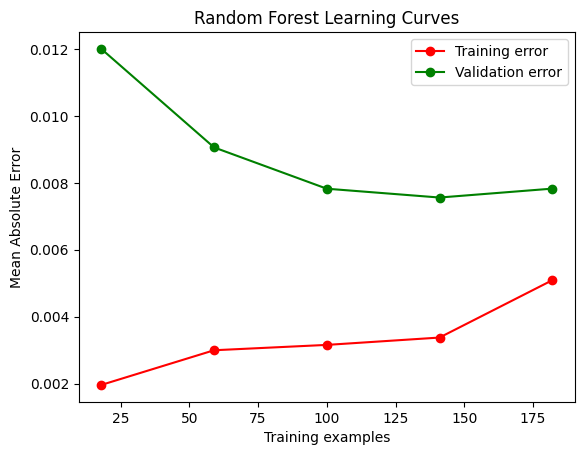
\includegraphics[width=\linewidth, trim=0 0 0 0]{images/RandomForest_lc80_ridotto.png} &
        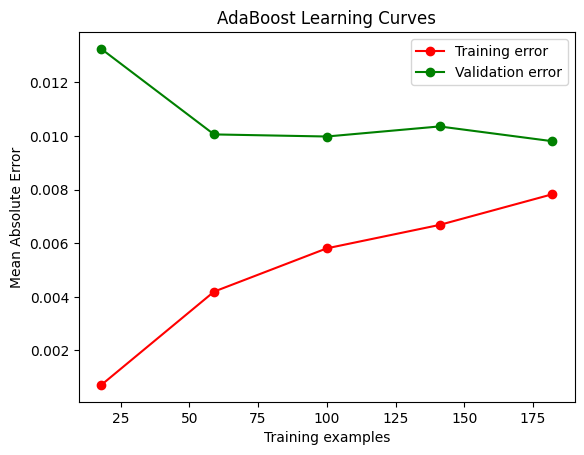
\includegraphics[width=\linewidth, trim=0 0 0 0]{images/AdaBoost_lc80_ridotto.png} \\
        \hline
    \end{tabularx}
    \caption{Learning Curves con dataset completo ridotto 80/20}
    \label{tab:emissions_info}
\end{table}

\noindent RandomForest sembrerebbe essere il migliore



\noindent\textbf{Split 90/10}


\begin{table}[H]
    \centering
    \begin{tabular}{|>{\centering\arraybackslash}m{5cm}|c|c|c|c|}
        \hline
        \textbf{Regressor} & \textbf{MAE} & \textbf{RMSE} & \textbf{MSLE} \\ [10pt]
        \hline
        SVR & 0.0296920 & 0.0011083 & 0.0010553 \\ [10pt]
        \hline
        Decision Tree & 0.0096568 & 0.0002100 & 0.0002000 \\ [10pt]
        \hline
        Random Forest & 0.0088683 & 0.0001676 & 0.0001582 \\ [10pt]
        \hline
        AdaBoost & 0.0115947 & 0.0002257 & 0.0002146 \\ [10pt]
        \hline
    \end{tabular}
    \caption{Risultati regressore con dataset completo ridotto 90/10}
    \label{tab:results}
\end{table}


\begin{table}[H]
    \centering
    \footnotesize
    \setlength\tabcolsep{0pt}
    \begin{tabularx}{\textwidth}{|X|X|}
        \hline
        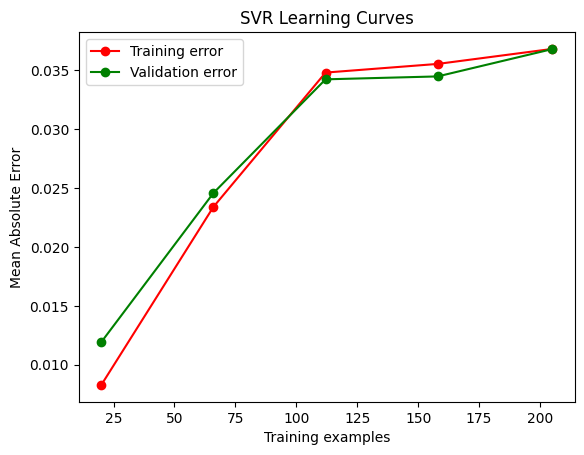
\includegraphics[width=\linewidth, trim=0 0 0 0]{images/SVR_lc90_ridotto.png} &
        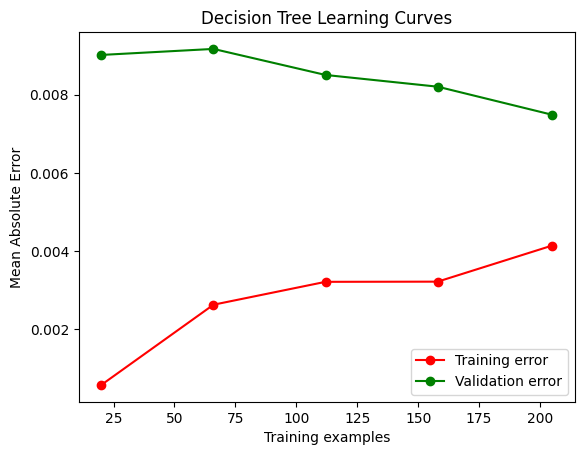
\includegraphics[width=\linewidth, trim=0 0 0 0]{images/DecisionTree_lc90_ridotto.png} \\
        \hline
        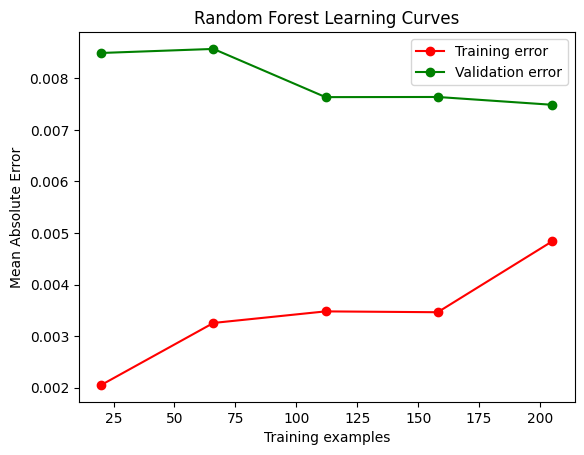
\includegraphics[width=\linewidth, trim=0 0 0 0]{images/RandomForest_lc90_ridotto.png} &
        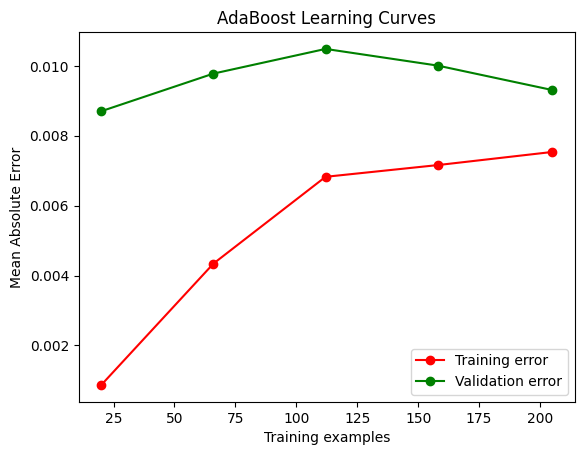
\includegraphics[width=\linewidth, trim=0 0 0 0]{images/AdaBoost_lc90_ridotto.png} \\
        \hline
    \end{tabularx}
    \caption{Learning Curves con dataset completo ridotto 90/10}
    \label{tab:emissions_info}
\end{table}

\noindent Il RandomForest sembrerebbe essere il migliore


\noindent
\textbf{Conclusioni}
Come si può notare in generale la riduzione del dataset ha portato a miglioramenti. Per quanto riguarda i diversi split si può notare che alcuni modelli performano meglio con alcuni split, altri modelli con altri. RandomForestRegressor risulta il migliore con lo split 60/40

\newpage

\subsubsection{Dataset AZURE}

\begin{figure}[H]
    \centering
    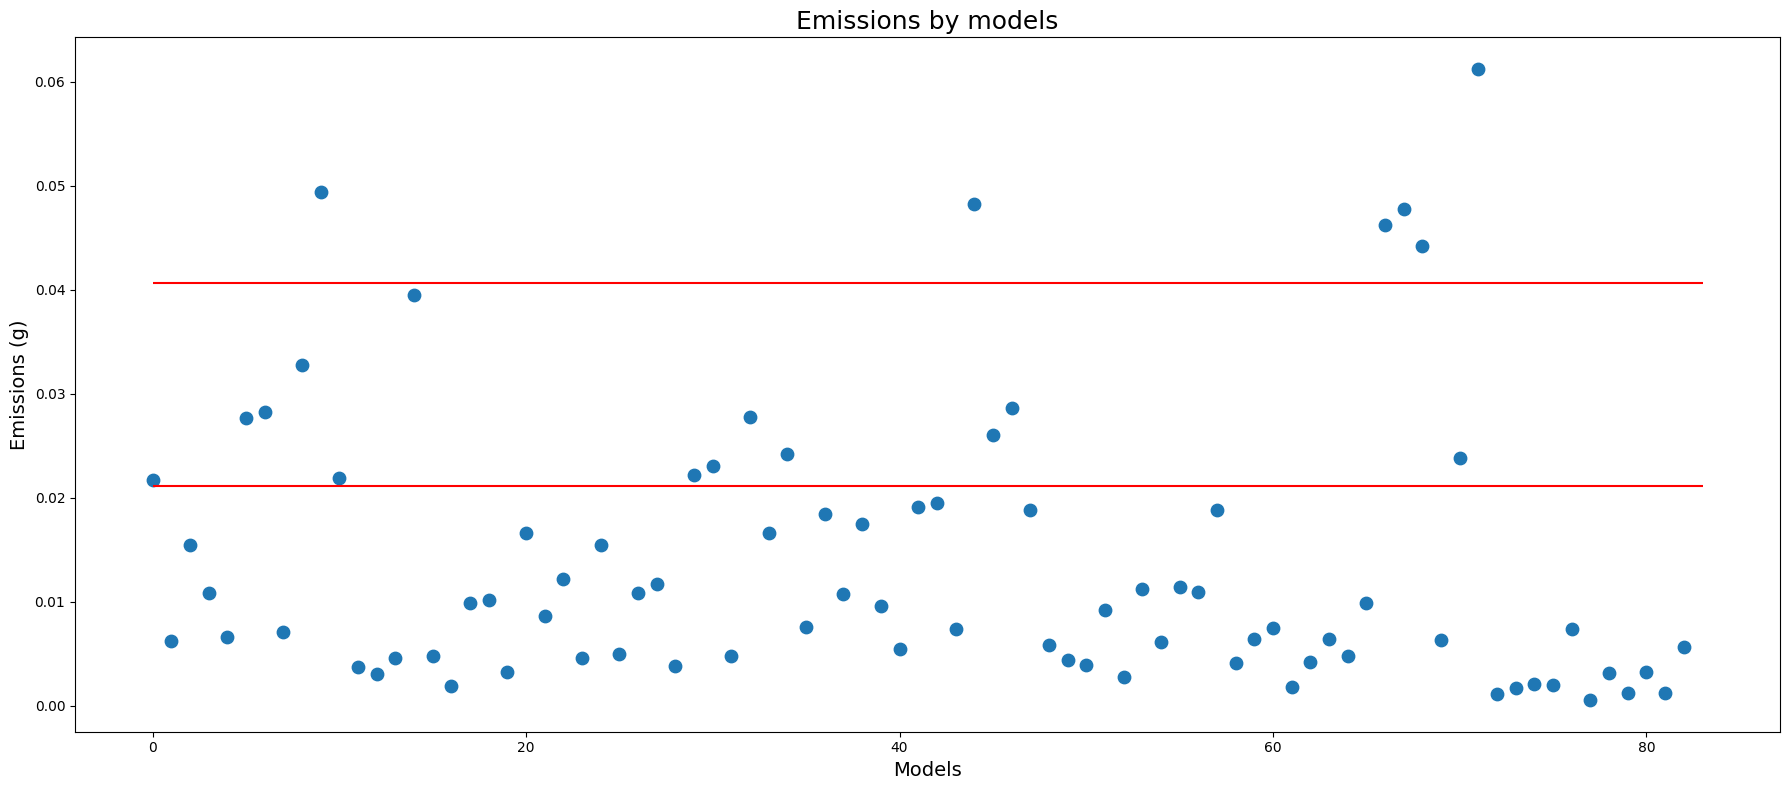
\includegraphics[scale=0.25]{images/nuova-situazione2-ridotto.png}
    \caption{Distribuzione delle emissioni nel dataset Azure ridotto}
\end{figure}


E’ possibile notare un miglior bilanciamento delle emissioni. Per quanto riguarda i modelli,
sono stati eseguti addestramenti con diversi split tra training e test set


\noindent\textbf{Split 50/50}


\begin{table}[H]
    \centering
    \begin{tabular}{|>{\centering\arraybackslash}m{5cm}|c|c|c|c|}
        \hline
        \textbf{Regressor} & \textbf{MAE} & \textbf{RMSE} & \textbf{MSLE} \\ [10pt]
        \hline
        SVR & 0.0201690 & 0.0004759 & 0.0004582 \\ [10pt]
        \hline
        Decision Tree & 0.0088806 & 0.0001921 & 0.0001823 \\ [10pt]
        \hline
        Random Forest & 0.0083870 & 0.0001706 & 0.0001619 \\ [10pt]
        \hline
        AdaBoost & 0.0087987 & 0.0001824 & 0.0001728 \\ [10pt]
        \hline
    \end{tabular}
    \caption{Risultati ottenuti con il dataset Azure ridotto 50/50}
    \label{tab:results}
\end{table}

\begin{table}[H]
    \centering
    \footnotesize
    \setlength\tabcolsep{0pt}
    \begin{tabularx}{\textwidth}{|X|X|}
        \hline
        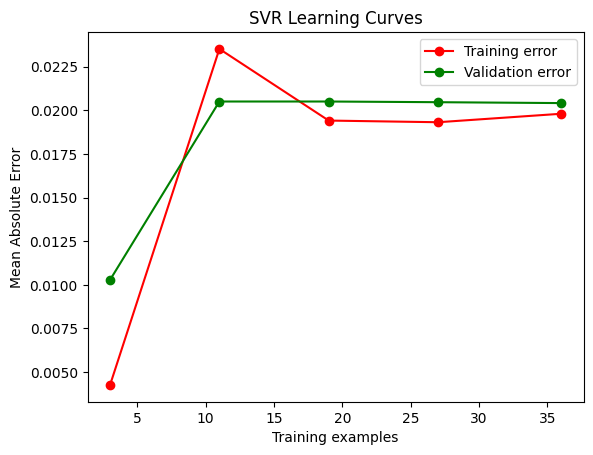
\includegraphics[width=\linewidth, trim=0 0 0 0]{images/SVR_lc50_ridottoAzure.png} &
        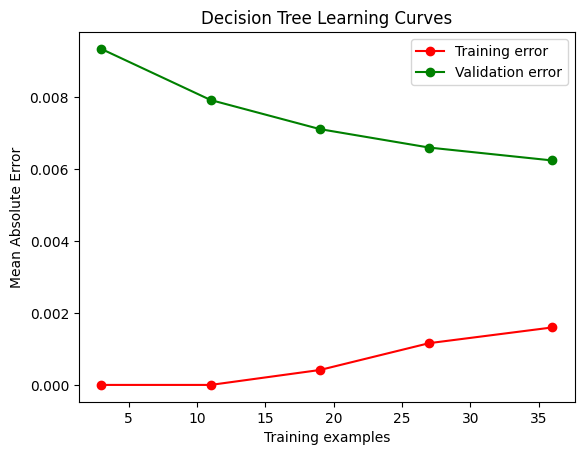
\includegraphics[width=\linewidth, trim=0 0 0 0]{images/DecisionTree_lc50_ridottoAzure.png} \\
        \hline
        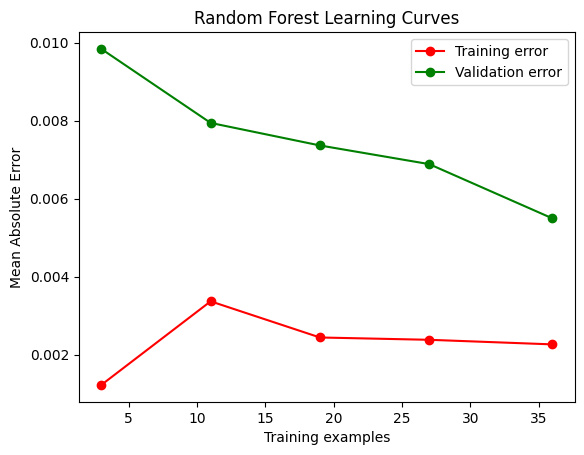
\includegraphics[width=\linewidth, trim=0 0 0 0]{images/RandomForest_lc50_ridottoAzure.png} &
        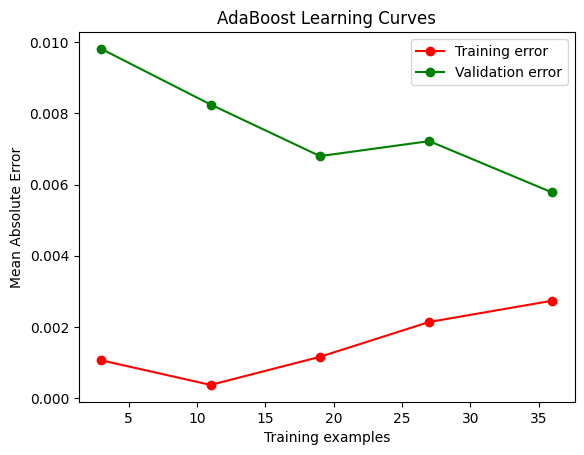
\includegraphics[width=\linewidth, trim=0 0 0 0]{images/AdaBoost_lc50_ridottoAzure.png} \\
        \hline
    \end{tabularx}
    \caption{Learning Curves con il dataset Azure ridotto 50/50}
    \label{tab:emissions_info}
\end{table}

\noindent RandomForest sembrerebbe essere il migliore

\noindent\textbf{Split 60/40}


\begin{table}[H]
    \centering
    \begin{tabular}{|>{\centering\arraybackslash}m{5cm}|c|c|c|c|}
        \hline
        \textbf{Regressor} & \textbf{MAE} & \textbf{RMSE} & \textbf{MSLE} \\ [10pt]
        \hline
        SVR & 0.0203710 & 0.0004819 & 0.0004645 \\ [10pt]
        \hline
        Decision Tree & 0.0079792 & 0.0001632 & 0.0001549 \\ [10pt]
        \hline
        Random Forest & 0.0076229 & 0.0001404 & 0.0001337 \\ [10pt]
        \hline
        AdaBoost & 0.0078253 & 0.0001293 & 0.0001236 \\ [10pt]
        \hline
    \end{tabular}
    \caption{Risultati ottenuti con il dataset Azure ridotto 60/40}
    \label{tab:results}
\end{table}

\begin{table}[H]
    \centering
    \footnotesize
    \setlength\tabcolsep{0pt}
    \begin{tabularx}{\textwidth}{|X|X|}
        \hline
        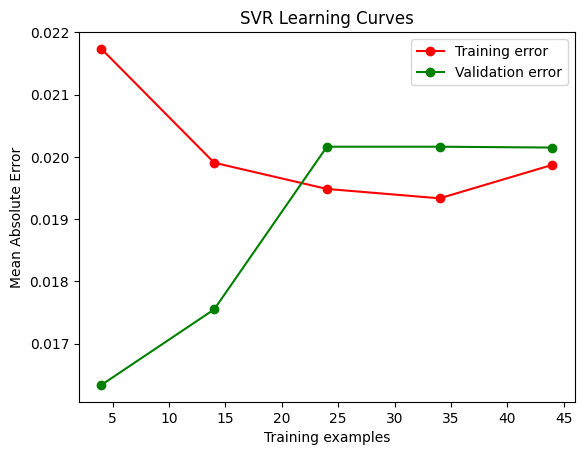
\includegraphics[width=\linewidth, trim=0 0 0 0]{images/SVR_lc60_ridottoAzure.png} &
        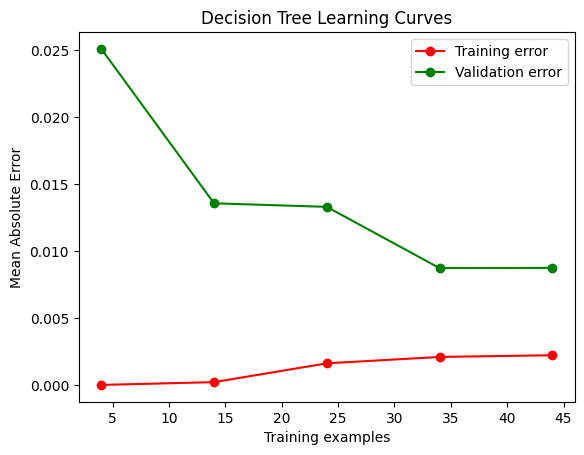
\includegraphics[width=\linewidth, trim=0 0 0 0]{images/DecisionTree_lc60_ridottoAzure.png} \\
        \hline
        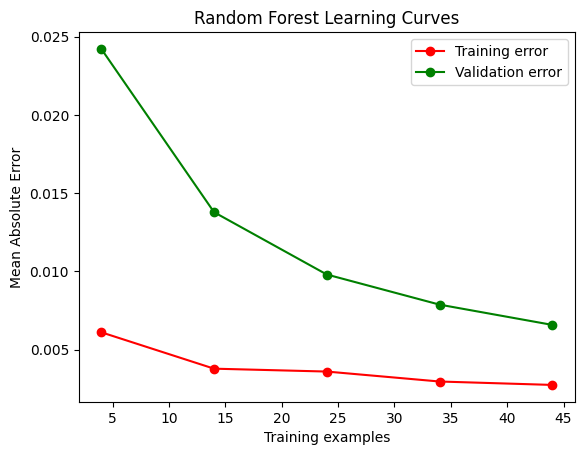
\includegraphics[width=\linewidth, trim=0 0 0 0]{images/RandomForest_lc60_ridottoAzure.png} &
        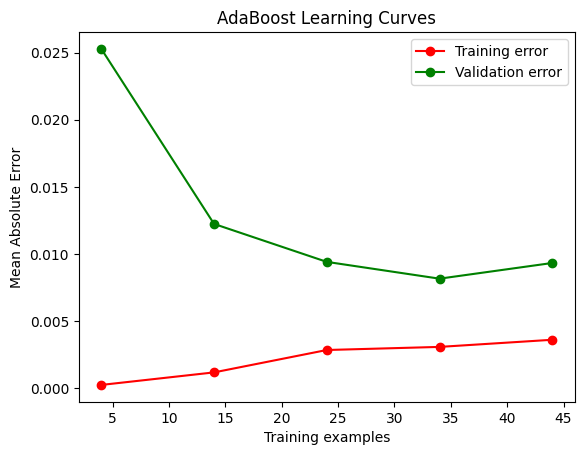
\includegraphics[width=\linewidth, trim=0 0 0 0]{images/AdaBoost_lc60_ridottoAzure.png} \\
        \hline
    \end{tabularx}
    \caption{Learning Curves con il dataset Azure ridotto 60/40}
    \label{tab:emissions_info}
\end{table}

\noindent RandomForest sembrerebbe essere il migliore


\noindent\textbf{Split 70/30}


\begin{table}[H]
    \centering
    \begin{tabular}{|>{\centering\arraybackslash}m{5cm}|c|c|c|c|}
        \hline
        \textbf{Regressor} & \textbf{MAE} & \textbf{RMSE} & \textbf{MSLE} \\ [10pt]
        \hline
        SVR & 0.0205812 & 0.0004825 & 0.0004649 \\ [10pt]
        \hline
        Decision Tree & 0.0086633 & 0.0001952 & 0.0001848 \\ [10pt]
        \hline
        Random Forest & 0.0079448 & 0.0001688 & 0.0001604 \\ [10pt]
        \hline
        AdaBoost & 0.0087171 & 0.0001541 & 0.0001471 \\ [10pt]
        \hline
    \end{tabular}
    \caption{Risultati ottenuti con il dataset Azure ridotto 70/30}
    \label{tab:results}
\end{table}

\begin{table}[H]
    \centering
    \footnotesize
    \setlength\tabcolsep{0pt}
    \begin{tabularx}{\textwidth}{|X|X|}
        \hline
        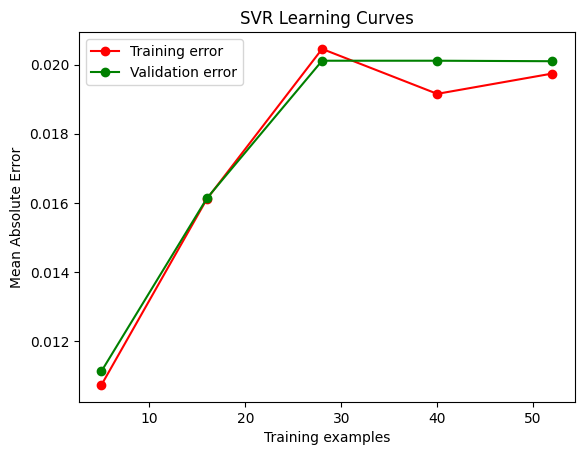
\includegraphics[width=\linewidth, trim=0 0 0 0]{images/SVR_lc70_ridottoAzure.png} &
        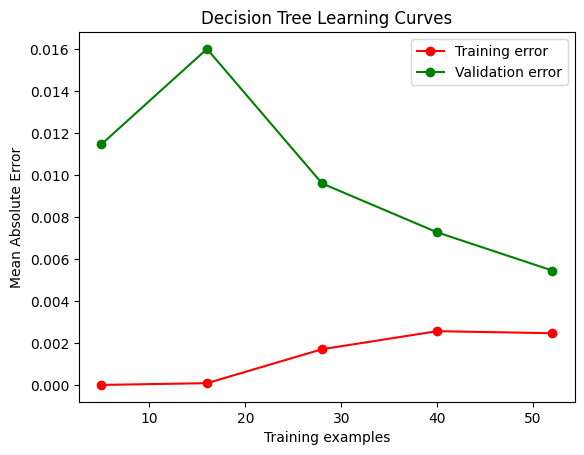
\includegraphics[width=\linewidth, trim=0 0 0 0]{images/DecisionTree_lc70_ridottoAzure.png} \\
        \hline
        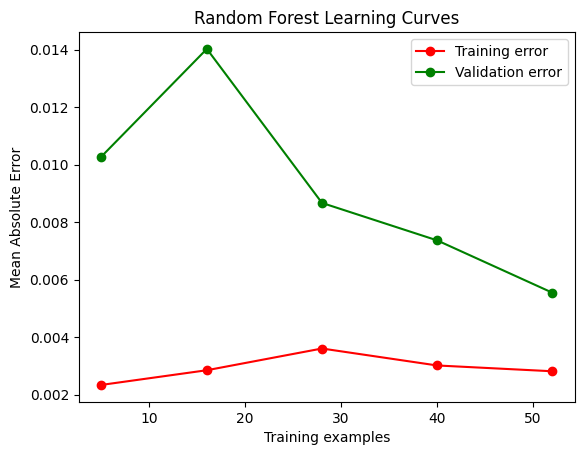
\includegraphics[width=\linewidth, trim=0 0 0 0]{images/RandomForest_lc70_ridottoAzure.png} &
        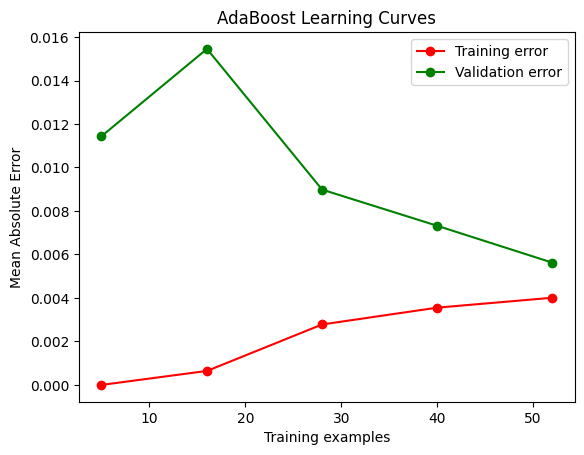
\includegraphics[width=\linewidth, trim=0 0 0 0]{images/AdaBoost_lc70_ridottoAzure.png} \\
        \hline
    \end{tabularx}
    \caption{Learning Curves con il dataset Azure ridotto 70/30}
    \label{tab:emissions_info}
\end{table}

\noindent AdaBoost sembrerebbe essere il migliore


\noindent\textbf{Split 80/20}


\begin{table}[H]
    \centering
    \begin{tabular}{|>{\centering\arraybackslash}m{5cm}|c|c|c|c|}
        \hline
        \textbf{Regressor} & \textbf{MAE} & \textbf{RMSE} & \textbf{MSLE} \\ [10pt]
        \hline
        SVR & 0.0207895 & 0.0004925 & 0.0004749 \\ [10pt]
        \hline
        Decision Tree & 0.0089766 & 0.0001894 & 0.0001786 \\ [10pt]
        \hline
        Random Forest & 0.0067808 & 0.0001078 & 0.0001032 \\ [10pt]
        \hline
        AdaBoost & 0.0076901 & 0.0001143 & 0.0001092 \\ [10pt]
        \hline
    \end{tabular}
    \caption{Risultati ottenuti con il dataset Azure ridotto 80/20}
    \label{tab:results}
\end{table}

\begin{table}[H]
    \centering
    \footnotesize
    \setlength\tabcolsep{0pt}
    \begin{tabularx}{\textwidth}{|X|X|}
        \hline
        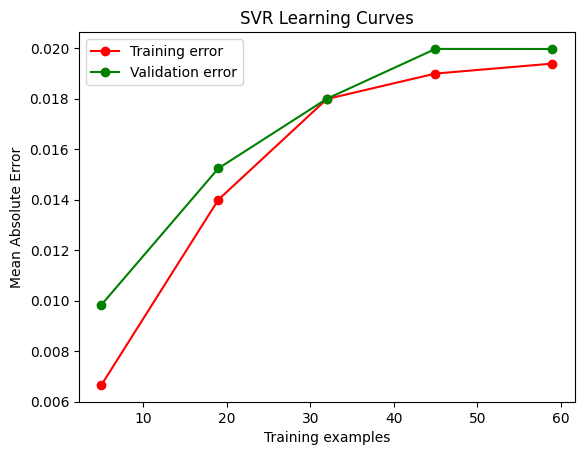
\includegraphics[width=\linewidth, trim=0 0 0 0]{images/SVR_lc80_ridottoAzure.png} &
        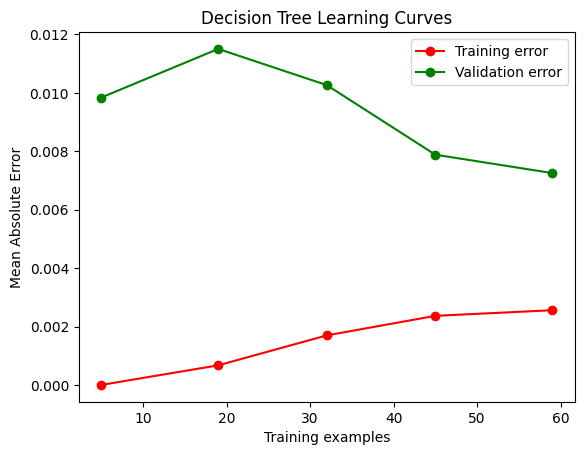
\includegraphics[width=\linewidth, trim=0 0 0 0]{images/DecisionTree_lc80_ridottoAzure.png} \\
        \hline
        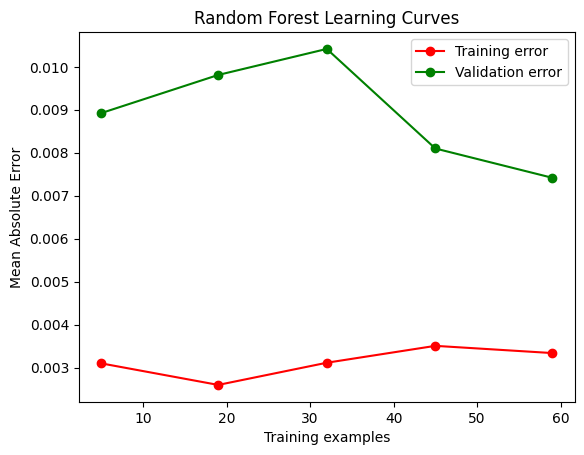
\includegraphics[width=\linewidth, trim=0 0 0 0]{images/RandomForest_lc80_ridottoAzure.png} &
        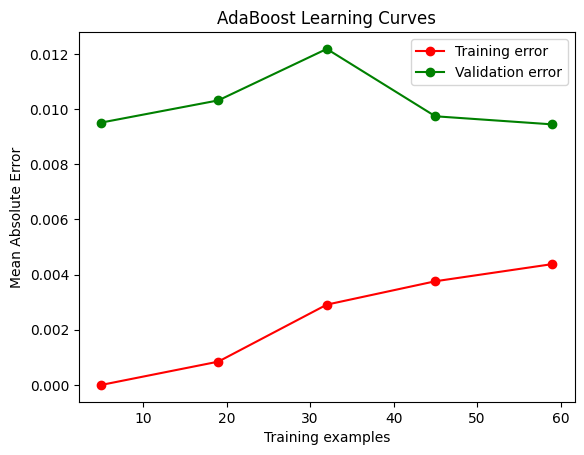
\includegraphics[width=\linewidth, trim=0 0 0 0]{images/AdaBoost_lc80_ridottoAzure.png} \\
        \hline
    \end{tabularx}
    \caption{Learning Curves con il dataset Azure ridotto 80/20}
    \label{tab:emissions_info}
\end{table}

\noindent RandomForest sembrerebbe essere il migliore



\noindent\textbf{Split 90/10}

\begin{table}[H]
    \centering
    \begin{tabular}{|>{\centering\arraybackslash}m{5cm}|c|c|c|c|}
        \hline
        \textbf{Regressor} & \textbf{MAE} & \textbf{RMSE} & \textbf{MSLE} \\ [10pt]
        \hline
        SVR & 0.0229610 & 0.0005560 & 0.0005361 \\ [10pt]
        \hline
        Decision Tree & 0.0049908 & 0.0000352 & 0.0000345 \\ [10pt]
        \hline
        Random Forest & 0.0045819 & 0.0000323 & 0.0000317 \\ [10pt]
        \hline
        AdaBoost & 0.0049257 & 0.0000379 & 0.0000371 \\ [10pt]
        \hline
    \end{tabular}
    \caption{Risultati ottenuti con il dataset Azure ridotto 90/10}
    \label{tab:results}
\end{table}


\begin{table}[H]
    \centering
    \footnotesize
    \setlength\tabcolsep{0pt}
    \begin{tabularx}{\textwidth}{|X|X|}
        \hline
        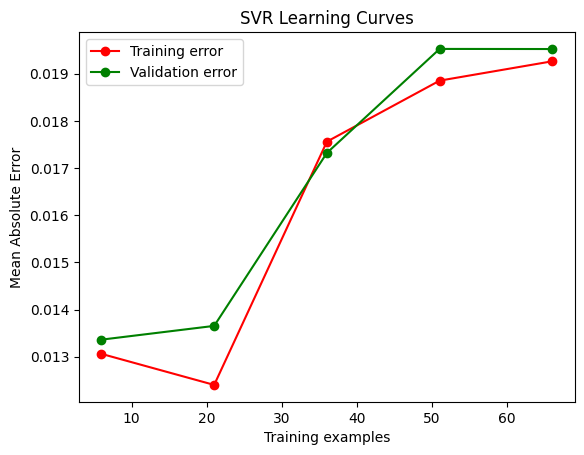
\includegraphics[width=\linewidth, trim=0 0 0 0]{images/SVR_lc90_ridottoAzure.png} &
        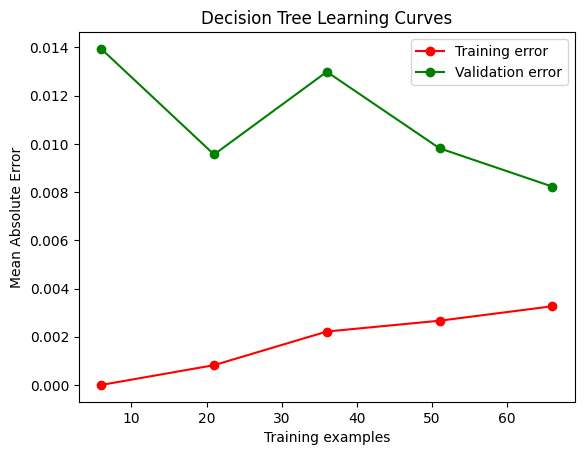
\includegraphics[width=\linewidth, trim=0 0 0 0]{images/DecisionTree_lc90_ridottoAzure.png} \\
        \hline
        \includegraphics[width=\linewidth, trim=0 0 0 0]{images/RandomForest_lc90_ridottoAzure.png} &
        \includegraphics[width=\linewidth, trim=0 0 0 0]{images/AdaBoost_lc90_ridottoAzure.png} \\
        \hline
    \end{tabularx}
    \caption{Learning Curves con il dataset Azure ridotto 90/10}
    \label{tab:emissions_info}
\end{table}

\noindent RandomForest sembrerebbe essere il migliore

\noindent\textbf{Conclusioni}
RandomForest sembra essere ancora il migliore.
Inoltre il dataset completo si comporta meglio rispetto a quello Azure senza e con riduzione